%% The first command in your LaTeX source must be the \documentclass command.
%%
%% Options:
%% twocolumn : Two column layout. Do not use twocolumn for papers submitted to CEUR-WS!
%% hf: enable header and footer.
\documentclass[
% twocolumn,
% hf,
]{ceurart}

%%
%% One can fix some overfulls
\sloppy

\usepackage[T1]{fontenc}
\usepackage{amsmath}
\usepackage{amssymb}
\usepackage{booktabs}
\usepackage{multirow}
\usepackage{caption}
\usepackage{tikz}
\usepackage{array}
\usepackage{xurl}
\usepackage{seqsplit}
\usepackage{microtype}
\usepackage{float}
\usepackage{placeins}

%%
%% Minted listings support
%% Need pygment <http://pygments.org/> <http://pypi.python.org/pypi/Pygments>
\usepackage{listings}
%% auto break lines
\lstset{breaklines=true}

\lstdefinestyle{pythoncode}{
  language=Python,
  basicstyle=\ttfamily\small,
  breaklines=true,
  frame=single,
  columns=fullflexible,
  showstringspaces=false,
  tabsize=2,
}
\lstdefinestyle{smvcode}{
  basicstyle=\ttfamily\small,
  breaklines=true,
  frame=single,
  columns=fullflexible,
  showstringspaces=false,
}
\lstset{basicstyle=\ttfamily\small}

%%
%% end of the preamble, start of the body of the document source.
\begin{document}

%%
%% Rights management information.
%% CC-BY is default license.
\copyrightyear{2026}
\copyrightclause{Copyright for this paper by its authors.
  Use permitted under Creative Commons License Attribution 4.0
  International (CC BY 4.0).}

%%
%% This command is for the conference information
\conference{ICTCS 2026: 27th Italian Conference on Theoretical Computer Science,
  September 07--09, 2026, Udine, Italy}

%%
%% The "title" command
\title{A verification pipeline for neuronal archetypes}

%%
%% The "author" command and its associated commands are used to define
%% the authors and their affiliations.
\author[1]{Thi-Thuy-Duong Pham}[%
orcid=0009-0006-4915-7465,
email=thi-thuy-duong.pham@etu.univ-cotedazur.fr,
url=https://github.com/thuyduong275,
]

\cormark[1]
\address[1]{I3S, CNRS, Université Côte d'Azur, Sophia Antipolis, France}

\author[1]{Elisabetta De Maria}[%
orcid=0000-0001-7116-9629,
email=elisabetta.de-maria@univ-cotedazur.fr,
]
\address[1]{I3S, CNRS, Université Côte d'Azur, Sophia Antipolis, France}

\author[2]{Robert De Simone}[%
orcid=0000-0002-3123-7591,
email=robert.de-simone@inria.fr,
]
\address[2]{Centre Inria d'Université Côte d'Azur, Sophia Antipolis, France}

%% Footnotes
\cortext[1]{Corresponding author.}

%%
%% The abstract is a short summary of the work to be presented in the
%% article.
\begin{abstract}
Spiking Neural Networks (SNNs) are considered to be more biologically realistic models of neural computation than traditional artificial neural networks, as they encode and process information through the timing of discrete spikes rather than continuous activation values. Within this framework, neuronal archetypes represent canonical connectivity patterns that serve as fundamental building blocks for constructing larger and more complex neural circuits. Understanding the dynamical properties of these archetypes is therefore a crucial first step toward explaining and predicting the behavior of the networks that emerge from their composition.

In this work, we propose a formal verification framework for analyzing the dynamics of neuronal archetypes through model checking. Our main contribution is the definition of a dedicated domain-specific language, named \textsc{NASL} (Neuronal Archetype Specification Language), to represent archetype structures and Leaky Integrate-and-Fire (LIF) neuron parameters, together with \texttt{snn\_mc}, an effective software tool support for the automatic translation and expansion of \textsc{NASL} specifications into discrete-time NuSMV models. Relevant dynamical properties are expressed in Computation Tree Logic (CTL) and Linear Temporal Logic (LTL) and verified exhaustively using the NuSMV model checker, which produces counterexample traces whenever a property is violated. Through representative archetype case studies, we demonstrate how this approach provides rigorous guarantees about archetype behavior and supports the systematic study of biologically inspired neural circuits. Finally, we discuss the extension of this framework toward the verification of archetype compositions, paving the way for the formal analysis of larger spiking neural networks built from these elementary structures.
\end{abstract}

%%
%% Keywords. The author(s) should pick words that accurately describe
%% the work being presented. Separate the keywords with commas.
\begin{keywords}
  Spiking Neural Networks \sep
  Neuronal Archetypes \sep
  Biological Neural Networks \sep
  Model Checking \sep
  Dynamic Properties
\end{keywords}

%%
%% This command processes the author and affiliation and title
%% information and builds the first part of the formatted document.
\maketitle

% =====================================================================
% SECTION 1 — INTRODUCTION
% =====================================================================
\section{Introduction}

Understanding the human brain remains one of the most profound challenges in
science. Biological neural networks exhibit highly complex dynamics that are
difficult to analyze through observation or simulation alone: experimental
manipulation of biological neural circuits is often infeasible or ethically
constrained, and exhaustive simulation of all possible behaviors of a network
rapidly becomes intractable as its size grows. Formal modelling and verification techniques offer a rigorous alternative,
providing a mathematical framework for abstracting neural systems and
exhaustively reasoning about their dynamics, rather than relying on a finite
set of simulated trajectories~\cite{Clarke1999}. Symbolic techniques in
particular have proved effective at taming the state-space explosion that
exhaustive verification would otherwise face, even for systems with very
large numbers of reachable states~\cite{Burch1994}.

A central obstacle to applying formal methods to neural systems lies in the
trade-off between biological realism and computational tractability. Highly
detailed models, such as the Hodgkin--Huxley model~\cite{Hodgkin1952},
capture a wide range of biological behaviors but are computationally
expensive, which limits their use in formal verification settings. Simplified
spiking neuron models, in particular the Leaky Integrate-and-Fire (LIF)
model~\cite{Lapicque1907,Gerstner2002}, retain the essential temporal
dynamics of spiking neural networks (SNNs) while remaining tractable enough
to be encoded as finite-state systems, making them well suited to model
checking.

Within the broader landscape of neural network models, SNNs are generally
regarded as the third generation, following the McCulloch--Pitts neuron, in
which units act as simple threshold logic gates~\cite{McCulloch1943}, and
continuous-activation models such as the multi-layer
perceptron~\cite{Cybenko1989}, whose outputs represent firing rates rather
than discrete spikes. Unlike these earlier generations, SNNs incorporate the
precise timing of individual spikes as an essential part of how information
is processed~\cite{Maass1997,PaugamMoisy2012}, which is what makes them
closer to biological neural systems and the focus of this work.

Rather than directly tackling large, intractable neural networks, this work
focuses on \emph{neuronal archetypes}~\cite{DeMaria2020}: small, recurrent
micro-circuits that represent canonical connectivity patterns commonly found
in biological neural systems, such as negative feedback loops and
contralateral inhibition. Neuronal archetypes act as fundamental building
blocks from which larger and more elaborate neural structures are composed.
Establishing rigorous guarantees on the dynamical behavior of individual
archetypes is therefore a necessary first step toward understanding, and
eventually verifying, the behavior of the larger networks that emerge from
their composition.

In this paper, we propose a formal verification framework for the automatic
analysis of neuronal archetypes through model checking, implemented in the
tool \texttt{snn\_mc}. Archetype topologies and LIF neuron parameters are
specified using \textsc{NASL} (Neuronal Archetype Specification Language),
a dedicated domain-specific language, automatically translated into a
discrete-time NuSMV~\cite{Cimatti1999} model. Relevant dynamical
properties, such as guaranteed oscillation or mutual exclusion between
competing neurons, are expressed in Computation Tree Logic
(CTL)~\cite{Clarke1986} and Linear Temporal Logic (LTL)~\cite{Pnueli1977},
and verified exhaustively using the NuSMV model checker, which produces a
counterexample trace whenever a property is violated. This pipeline allows
archetype behavior to be specified, modelled, and verified without manual
intervention at the model-checking level, and is illustrated through a
representative archetype case study.

Several works have applied formal verification techniques to spiking neural
networks. Some studies map spiking neural P systems into timed automata to
analyze their temporal properties~\cite{Aman2016}; others use timed
automata to model LIF neural networks and verify system behaviors using
temporal logic formulas~\cite{DeMaria2018}. De Maria et
al.~\cite{DeMaria2020} propose a formal framework for modelling and verifying
neuronal archetypes using Lustre, a synchronous language, to encode neurons
and neuronal graphs and to express temporal properties concerning their
dynamic behavior, subsequently verified by model checkers. Beyond
deterministic models, Yao et al.~\cite{yao2023probabilistic} propose a formal framework
for modelling and verifying probabilistic SNNs, in which synaptic
transmission and spike generation are governed by stochastic processes,
combining probabilistic model checking with a biologically grounded neuron
model to verify quantitative properties such as the probability of a neuron
firing within a given time window. These formal approaches, both
deterministic and probabilistic, provide a systematic way to reason about
neural computation; our work builds on this line of research by targeting an
automated, DSL-driven pipeline for the verification of neuronal archetypes
using NuSMV.

The remainder of this paper is organized as follows. Section~\ref{sec:preliminaries}
introduces the necessary background on the LIF neuron model, temporal logics,
the NuSMV model checker, and neuronal archetypes. Section~\ref{sec:pipeline}
presents the proposed verification pipeline, from the DSL specification to
NuSMV model generation, property generation, and verification.
Section~\ref{sec:case-study} illustrates this pipeline on a representative
archetype case study. Finally, Section~\ref{sec:conclusion} concludes the
paper and discusses the extension of this framework toward the verification
of archetype compositions.

% =====================================================================
% SECTION 2 — PRELIMINARIES
% =====================================================================
\section{Preliminaries}
\label{sec:preliminaries}

This section introduces the biological and theoretical background needed throughout the paper.

\subsection{Leaky Integrate-and-Fire Neuron Model}
\label{sec:lif}

The Leaky Integrate-and-Fire (LIF) model is a simplified computational model
that captures the essential behavior of biological neurons while remaining
computationally efficient~\cite{Lapicque1907,Gerstner2002}. A neuron
accumulates excitatory and inhibitory post-synaptic potentials through
spatial summation (across synapses) and temporal summation (over time); its
membrane potential also decays through a leakage effect, and a spike is
emitted whenever the potential exceeds a threshold~\cite{DeMaria2020,Gerstner2002,Purves2006}.

A LIF is represented as a weighted directed graph,
$(V, E, w)$, where $V$ is the set of neurons, $E \subseteq V \times V$
represents synaptic connections, and $w : E \to \mathbb{Z}$ assigns an
integer synaptic strength to each edge, measured in membrane-potential units
within $[0, P_{max}]$: a positive weight corresponds to excitation, a
negative weight to inhibition~\cite{DeMaria2020}.

Each neuron is characterized by a tuple $(\tau, r, p, y)$, where $\tau$ is the
firing threshold, $r$ is the leak factor, $p(t)$ the membrane potential
at time $t$, and $y(t)$ the neuron output~\cite{Lapicque1907,DeMaria2020}.
Following De Maria et al.~\cite{DeMaria2020}, temporal summation is captured
by a bounded sliding window of length $\sigma$, where
\[
p(t)=\sum_{e=0}^{\sigma} r^{e}\sum_{i=1}^{m} w_i x_i(t-e),
\]
and $x_i(t)\in\{0,1\}$ denotes the input spike from neuron $i$.

\subsection{Neuronal Archetypes}
\label{sec:archetypes}

Neuronal archetypes are elementary neuronal circuits composed of a small
number of neurons, each fulfilling a specific computational
function~\cite{DeMaria2020}. The central hypothesis is that any neuronal
micro-circuit, regardless of its size or topological complexity, can be
reduced to one of a finite set of such archetypes, which can further be
coupled---by connecting outputs to inputs or by nesting---to form more
elaborate functional structures~\cite{DeMaria2020,DeMaria2017}. We consider
the six fundamental motifs from De Maria et al.~\cite{DeMaria2020}
illustrated in Figure~\ref{fig:archetypes}(a--f), together with a seventh
positive feedback loop extension (g):\emph{simple series}, a chain where each neuron receives the output of its
predecessor; \emph{series with multiple outputs}, a series whose every
neuron's output is observed at each time step; \emph{parallel composition},
a set of neurons driven by a single common input neuron; \emph{negative
loop}, two neurons where the first excites the second and the second
inhibits the first, producing oscillatory behavior; \emph{inhibition of a
behavior}, two neurons where the first suppresses the activity of the
second; \emph{contralateral inhibition}, two or more neurons that mutually
inhibit one another, giving a winner-takes-all dynamic; and \emph{positive
loop}, an excitatory ring that can sustain reverberatory activity when the
loop gain exceeds threshold.

\begin{figure}[h]
    \centering
    % --- Top row: (a), (b), (c) ---
    \begin{tabular}{@{}c@{\hspace{0.6cm}}c@{\hspace{0.6cm}}c@{}}
        % (a) Simple series
        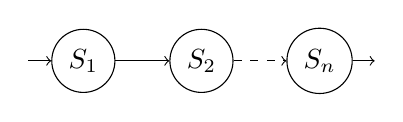
\begin{tikzpicture}
            \node[circle, draw] (s1) at (0,0) {$S_1$};
            \node[circle, draw] (s2) at (1.5,0) {$S_2$};
            \node[circle, draw] (sn) at (3,0) {$S_n$};
            \draw[->] (-0.7,0) -- (s1);
            \draw[->] (s1) -- (s2);
            \draw[dashed, ->] (s2) -- (sn);
            \draw[->] (sn) -- (3.7,0);
        \end{tikzpicture}
        &
        % (b) Series with multiple outputs (cascading, L-shaped links)
        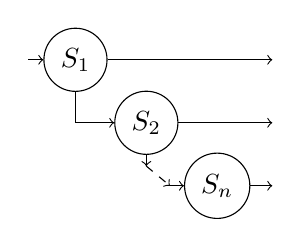
\begin{tikzpicture}
            \node[circle, draw] (s1) at (0, 0.8) {$S_1$};
            \node[circle, draw] (s2) at (0.9, 0) {$S_2$};
            \node[circle, draw] (sn) at (1.8, -0.8) {$S_n$};
            \draw[->] (-0.6, 0.8) -- (s1.west);
            \draw[->] (s1.east) -- (2.5, 0.8);
            \draw[->] (s1.south) |- (s2.west);
            \draw[->] (s2.east) -- (2.5, 0);
            \draw[->] (s2.south) -- (0.9, -0.55);
            \draw[dashed, ->] (0.9, -0.55) -- (1.2, -0.8);
            \draw[->] (1.2, -0.8) -- (sn.west);
            \draw[->] (sn.east) -- (2.5, -0.8);
        \end{tikzpicture}
        &
        % (c) Parallel composition
        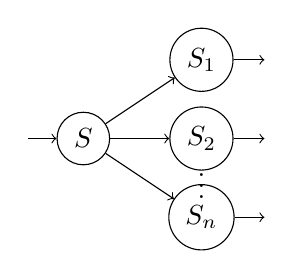
\begin{tikzpicture}
            \node[circle, draw] (s)  at (0,0)   {$S$};
            \node[circle, draw] (s1) at (1.5,1) {$S_1$};
            \node[circle, draw] (s2) at (1.5,0) {$S_2$};
            \node[circle, draw] (sn) at (1.5,-1){$S_n$};
            \draw[->] (-0.7,0) -- (s);
            \draw[->] (s) -- (s1);
            \draw[->] (s) -- (s2);
            \draw[->] (s) -- (sn);
            \draw[->] (s1) -- (2.3,1);
            \draw[->] (s2) -- (2.3,0);
            \draw[->] (sn) -- (2.3,-1);
            \node at (1.5,-0.5) {\vdots};
        \end{tikzpicture}
        \\[0.25cm]
        (a) Simple series &
        (b) Series with multiple outputs &
        (c) Parallel composition
    \end{tabular}
    \\[0.4cm]
    % --- Bottom row: (d), (e), (f), (g) ---
    \begin{tabular}{@{}c@{\hspace{0.45cm}}c@{\hspace{0.45cm}}c@{\hspace{0.45cm}}c@{}}
        % (d) Negative loop
        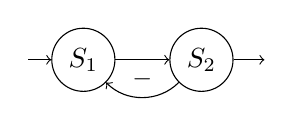
\begin{tikzpicture}
            \node[circle, draw] (s1) at (0,0) {$S_1$};
            \node[circle, draw] (s2) at (1.5,0) {$S_2$};
            \draw[->] (-0.7,0) -- (s1);
            \draw[->] (s1) -- (s2);
            \draw[->] (s2) -- (2.3,0);
            \draw[->, bend left=45] (s2) to
                node[above]{\small$-$} (s1);
        \end{tikzpicture}
        &
        % (e) Inhibition of a behavior
        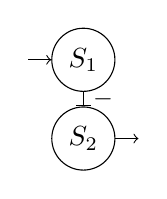
\begin{tikzpicture}
            \node[circle, draw] (s1) at (0,0.5) {$S_1$};
            \node[circle, draw] (s2) at (0,-0.5) {$S_2$};
            \draw[->] (-0.7,0.5) -- (s1);
            \draw[-|] (s1) -- node[right]{\small$-$} (s2);
            \draw[->] (s2) -- (0.7,-0.5);
        \end{tikzpicture}
        &
        % (f) Contralateral inhibition
        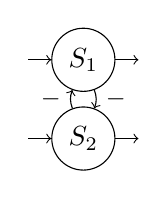
\begin{tikzpicture}
            \node[circle, draw] (s1) at (0,0.5) {$S_1$};
            \node[circle, draw] (s2) at (0,-0.5) {$S_2$};
            \draw[->] (-0.7,0.5) -- (s1);
            \draw[->] (-0.7,-0.5) -- (s2);
            \draw[->, bend left=20] (s1) to
                node[right]{\small$-$} (s2);
            \draw[->, bend left=20] (s2) to
                node[left]{\small$-$} (s1);
            \draw[->] (s1) -- (0.7,0.5);
            \draw[->] (s2) -- (0.7,-0.5);
        \end{tikzpicture}
        &
        % (g) Positive loop
        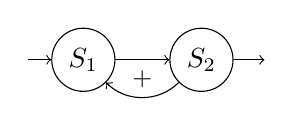
\begin{tikzpicture}
            \node[circle, draw] (s1) at (0,0) {$S_1$};
            \node[circle, draw] (s2) at (1.5,0) {$S_2$};
            \draw[->] (-0.7,0) -- (s1);
            \draw[->] (s1) -- (s2);
            \draw[->] (s2) -- (2.3,0);
            \draw[->, bend left=45] (s2) to
                node[above]{\small$+$} (s1);
        \end{tikzpicture}
        \\[0.25cm]
        (d) Negative loop &
        (e) Inhibition of a behavior &
        (f) Contralateral inhibition &
        (g) Positive loop
    \end{tabular}
    \caption{The six fundamental neuronal archetypes (a--f), adapted
    from~\cite{DeMaria2020}, together with the positive feedback loop
    extension (g).}
    \label{fig:archetypes}
\end{figure}


These archetypes are biologically inspired logical operators,
easily adjustable by tuning a small number of parameters, and
they constitute the basis of typical instances of neuronal
information processing~\cite{DeMaria2020}.

\subsection{Temporal Logic and Model Checking}
\label{sec:tl-mc}

The behavior of a discretized LI\&F network can be represented as a
transition system~\cite{Clarke1999}, defined as the tuple
$T=(S,S_0,\Sigma,\rightarrow,AP,L)$, where $S$ is the finite set of
reachable states, $S_0 \subseteq S$ is the set of initial states,
$\Sigma$ is the set of input symbols (or actions), $\rightarrow \subseteq
S \times \Sigma \times S$ is the transition relation, $AP$ is the set of
atomic propositions, and $L:S \rightarrow 2^{AP}$ is the labeling
function. In our model, each state represents the membrane potentials and
spike emission statuses of all neurons at a given discrete time instant,
while each transition corresponds to one evolution step according to the
$\sigma$-window LI\&F encoding described in
Section~\ref{sec:lif}. Since $\sigma$, $P_{max}$, and the integer synaptic
weights are bounded, the resulting state space is finite, making the
system amenable to automatic verification~\cite{DeMaria2016,DeMaria2017}.

Two major temporal logics are used to express dynamical
properties~\cite{Clarke1999}: Computation Tree Logic
(CTL)~\cite{Clarke1986}, which interprets formulas over the branching-time
structure of computation by pairing each temporal operator (\texttt{X},
\texttt{F}, \texttt{G}, \texttt{U}) with a path quantifier \texttt{A} (all
paths) or \texttt{E} (some path) and Linear Temporal Logic (LTL)~\cite{Pnueli1977}, evaluated over
a single infinite execution without explicit path quantifiers.

Model checking automatically verifies whether a transition system $T$
satisfies a formula $\varphi$, written $T \models \varphi$, by exhaustively
exploring all reachable states. When a property does not hold, the
model checker produces a counterexample trace witnessing the violation.

\subsection{NuSMV}
\label{sec:nusmv}

NuSMV~\cite{Cimatti1999} is a widely used symbolic model checker built on
Binary Decision Diagrams (BDDs), supporting the verification of finite-state
systems against specifications written in both CTL and LTL. A NuSMV model is
described in a dedicated input language organized into modules, each
declaring a set of state variables, an initial condition, and a transition
relation that updates these variables at every discrete time step;
properties to be verified are declared separately, using the
\texttt{CTLSPEC} and \texttt{LTLSPEC} keywords. This modular structure makes
NuSMV well suited to encoding the discrete states, recursive membrane
potential equations, and threshold-triggered transitions of the LIF neuron
model introduced in Section~\ref{sec:lif}.

% =====================================================================
% SECTION 3 — VERIFICATION PIPELINE (văn phong tự nhiên hơn, giữ đầy đủ nội dung)
% =====================================================================
\section{Verification Pipeline for Spiking Neural Network Models}
\label{sec:pipeline}

To practically evaluate the theoretical framework of
Section~\ref{sec:preliminaries}, we developed \texttt{snn\_mc}, an automated
tool that implements a linear verification pipeline for spiking neural
networks, bridging \emph{formal modelling}, \emph{DSL compilation}, and
\emph{model checking}. The tool takes a high-level archetype description
written in \textsc{NASL}, our domain-specific language, compiles it into a
discrete-time NuSMV model together with temporal specifications
(CTLSPEC/LTLSPEC), invokes the NuSMV model checker
(Section~\ref{sec:nusmv}), and summarises the results. This workflow
reflects the formal approach of~\cite{DeMaria2020,DeMaria2016,DeMaria2017},
and the whole process is fully automated behind a single command-line
invocation.

\subsection{System Overview and Execution Workflow}
\label{sec:overview}

The system is designed as a two-stage pipeline, following the classical
formal verification workflow \emph{system specification} $\rightarrow$
\emph{model construction} $\rightarrow$ \emph{property verification}:
\begin{itemize}
\item \textbf{Stage~1 --- Model Generation:} A \textsc{NASL} specification
      describes the structure and dynamics of a neural network; it is
      compiled into a finite-state transition system encoded in the
      \texttt{.smv} format accepted by NuSMV~\cite{Cimatti1999}.
\item \textbf{Stage~2 --- Model Checking:} The generated model is executed
      in NuSMV to verify temporal logic properties expressed in CTL or LTL.
      NuSMV reports whether each property holds and, when it does not,
      produces a counterexample trace for analysis.
\end{itemize}
All stages are orchestrated by \texttt{main()} in \texttt{snn\_mc/cli.py},
which is the unique entry point. Each module stays passive when imported
and is only invoked by this orchestration layer. From the user's
perspective, the entire process is triggered by a single command,
\texttt{python -m snn\_mc run <file.dsl> --out <dir>}, which (1) reads the
\textsc{NASL} file, (2) compiles it into a formal NuSMV model and property
file, (3) executes the combined model in NuSMV (Section~\ref{sec:nusmv}),
and (4) collects and summarises the verification results, including the
number of satisfied and violated properties and detailed logs for
debugging. This automation removes any need for manual interaction with
the model checker. Listing~\ref{lst:cli-main} shows the core processing
chain. The complete source code of \texttt{snn\_mc}, including the
\textsc{NASL} grammar, the example archetype specifications, and the case
study presented in Section~\ref{sec:case-study}, is publicly available at
\url{https://github.com/thuyduong275/neuro-archetype-verification-pipeline}.

\begin{lstlisting}[style=pythoncode,caption={Core orchestration in \texttt{snn\_mc/cli.py}.},label=lst:cli-main]
ir = composer.compose(parse_file(dsl, override_n=override_n))
prepared = smv.prepare_ir(ir)
combined_path.write_text(smv.build_combined_smv(ir, prepared, ...))
nusmv_rc, log_text = run_nusmv(combined_path, log_path, ...)
summary = summarize_nusmv_output(log_text)
\end{lstlisting}

\FloatBarrier
\begin{figure}[!ht]
\centering

\includegraphics[width=0.7\linewidth]{Fig/pipeline_flowchart.png}
\caption{Processing workflow of the \texttt{snn\_mc} system: from the input
\textsc{NASL} file to the output artefacts. Each numbered stage corresponds
to one step in the pipeline.}
\label{fig:pipeline_flow}
\end{figure}
\FloatBarrier

Figure~\ref{fig:pipeline_flow} illustrates the complete processing workflow
from the input \texttt{.dsl} file to the output artefacts written on disk.
Solid arrows represent the main control flow; dashed arrows represent
intermediate data structures or files on disk. The following subsections
describe the compilation stages in detail; the end-to-end execution
process, including reporting and simulation support, is summarised in
Section~\ref{subsec:end-to-end}.



\subsection{Compilation from DSL to Formal Model}
\label{sec:compilation}

The transformation from \textsc{NASL} to a formal model is the core
component of the system, since it directly impacts the correctness and
expressiveness of the verification process.

\subsubsection{Neural Network Representation}

The internal representation must capture both topology and LIF dynamics in
a form suitable for NuSMV code generation. The neural network is stored as
a directed graph: nodes represent neurons and external inputs, and edges
represent weighted synaptic connections, where a positive weight means
excitation and a negative weight means inhibition, consistent with the
weighted-graph definition of Section~\ref{sec:lif}. Beyond individual
edges, the system introduces \emph{archetypes}, the canonical structural
motifs that bridge these biological patterns with the automatic property
templates emitted later in the pipeline.

\subsubsection{DSL Parsing and Consistency Checking}

The parser in \texttt{snn\_mc/dsl/parser.py} reads one \textsc{NASL}
statement per line (\texttt{\#} starts a comment), expands \texttt{include}
directives, and builds a \texttt{NetworkIR} object containing neurons,
\texttt{Edge} objects, LIF parameter sets, input schedules, composition
declarations, user \texttt{spec} lines, and explicit \texttt{block}
archetype instances. When the parser encounters
\texttt{block <kind> key=value ...}, it looks up \texttt{BLOCK\_REGISTRY}
and calls \texttt{apply\_block()} on the matching archetype class, which
expands the macro into neurons and edges at parse time.
Table~\ref{tab:dsl-statements} summarises the core \textsc{NASL}
statements. After parsing, \texttt{compose()} in
\texttt{snn\_mc/composer.py} performs semantic validation without changing
the topology: every \texttt{input=} in a block must refer to a declared
input or an already existing neuron, so chaining \texttt{block
simple\_series} before \texttt{block negative\_loop input=c4} works as
expected. This early validation catches wiring errors at the
\textsc{NASL} level, before any NuSMV text is generated, which avoids
opaque SMV syntax failures during verification later on.
Listing~\ref{lst:dsl-syntax} shows the parser's entry point and the
block-expansion call it triggers.

\FloatBarrier
\begin{table}[!ht]
\centering
\caption{Core statements of \textsc{NASL}, the \texttt{snn\_mc} domain-specific language.}
\label{tab:dsl-statements}
\begin{tabular}{@{}ll@{}}
\toprule
\textbf{Statement} & \textbf{Meaning} \\
\midrule
\texttt{include <file>} & Inline another \textsc{NASL} file \\
\texttt{horizon <int>} & Clock \texttt{t} ranges \texttt{0..horizon} \\
\texttt{input <name>} & External Boolean stimulus \\
\texttt{schedule <in> values ...} & Fixed input prefix (then nondeterministic) \\
\texttt{neuron\_params <name> ...} & LIF bundle $(\tau, w_{exc}, w_{inh}, S, R, P_{max})$ \\
\texttt{block <kind> key=value} & Archetype macro (neurons + edges) \\
\texttt{edge / exc / inh} & Manual weighted synapse \\
\texttt{compose seq|par ...} & Explicit composition between neurons \\
\texttt{spec CTLSPEC|LTLSPEC ...} & User-provided temporal property \\
\bottomrule
\end{tabular}
\end{table}

\begin{lstlisting}[style=pythoncode,caption={Parser entry point and block expansion.},label=lst:dsl-syntax]
# block <kind> key=value ...  -> BLOCK_REGISTRY[kind].apply_block(...)
ir = parse_file(dsl_path, override_n=override_n)  # -> NetworkIR
ir = composer.compose(ir)  # semantic validation only
\end{lstlisting}

\subsubsection{Identifier Sanitization and SMV Preparation}

\texttt{prepare\_ir()} in \texttt{snn\_mc/smv/prepare.py} produces a
NuSMV-safe snapshot, \texttt{SmvPrepared}, that is shared by all code
generators. It sanitises every neuron and input name via
\texttt{sanitize\_identifier()} to avoid clashes with NuSMV reserved
keywords, and propagates the renames to edges, schedules, compositions,
and user spec text. Edges are grouped per neuron into excitatory
(\texttt{exc\_srcs}) and inhibitory (\texttt{inh\_srcs}) source lists,
reflecting spatial summation at each synapse. Explicit archetypes from
\textsc{NASL} \texttt{block} lines are merged with graph-detected
instances from \texttt{detect\_archetypes}, deduplicated by kind and node
set. Because the snapshot is a single immutable object, the model and
property emitters that come after it always refer to the same renamed
graph. Listing~\ref{lst:prepare-ir} shows the identifier-sanitisation
mapping and the resulting archetype list.

\begin{lstlisting}[style=pythoncode,caption={Preparation: sanitisation and archetype merge.},label=lst:prepare-ir]
mapping = {n: sanitize_identifier(n) for n in all_names}
arch_list = _build_arch_list(archetypes, neurons, inputs, edges)
\end{lstlisting}

\subsubsection{Automatic Archetype Detection}

\texttt{detect\_archetypes()} in \texttt{snn\_mc/archetypes/\_\_init\_\_.py}
automatically identifies structural motifs from the network graph when users
define neuron connections manually instead of using \texttt{block} macros. It
constructs a \texttt{GraphIndex} representation and applies a sequence of
detection heuristics following the predefined
\texttt{DETECTION\_ORDER}. Detected motifs are then mapped to the same
verification property templates used by explicitly declared
\texttt{block} macros, allowing manually defined networks and block-based
specifications to share the same verification workflow.
Seven block types are registered in \texttt{BLOCK\_REGISTRY}, including
\texttt{positive\_loop} and \texttt{series\_multiple\_outputs} as
practical extensions beyond the six motifs of Fig.~\ref{fig:archetypes}.
Detection links manual edge declarations to the same property templates
used by explicit \texttt{block} macros, so that a manually wired network
and a block-based one share the same verification workflow while still
preserving formal guarantees. Listing~\ref{lst:block-registry} lists the
registered archetype classes in the fixed detection order applied by the
tool.

\begin{lstlisting}[style=pythoncode,caption={Archetype registry and detection order.},label=lst:block-registry]
DETECTION_ORDER = (NegativeLoopArchetype, ContralateralInhibitionArchetype,
                    InhibitionOfBehaviorArchetype, ParallelCompositionArchetype,
                    SimpleSeriesArchetype)
\end{lstlisting}

\subsubsection{Automatic Property Generation}

\texttt{emit\_properties\_block()} in \texttt{snn\_mc/smv/properties.py}
emits temporal logic specifications that characterise archetype behaviour,
so the user does not have to write every formula by hand. It always
appends specs in a stable four-block order: (1)~baseline LIF invariants
per neuron (reset on spike, $P$ within bounds, spike--threshold
equivalence, fixed leak factor); (2)~composition properties from explicit
or inferred \texttt{compose} declarations; (3)~archetype templates from
\texttt{archetype\_specs()} for each entry in \texttt{arch\_list}; and
(4)~the user's verbatim \texttt{spec} lines. Listing~\ref{lst:properties-order}
shows the core loop that appends the archetype-specific templates for
each detected or declared instance.

\begin{lstlisting}[style=pythoncode,caption={Property emission order in \texttt{properties.py}.},label=lst:properties-order]
for it in dedup_archetype_instances(arch_list):
    auto.extend(archetype_specs(it, neurons=prepared.neurons, horizon=ir.horizon))
\end{lstlisting}

\subsubsection{NuSMV Model Generation}

\texttt{smv/model.py} emits \texttt{MODULE main} with the global clock,
input schedules, per-edge weighted sums (\texttt{net\_exc},
\texttt{net\_inh}), and the neuron instances. \texttt{smv/lif\_module.py}
defines \texttt{MODULE lif\_<pset>}, which implements the
leak--integrate--fire update with a fixed leak factor $R/S$ per parameter
set, and \texttt{smv/combined.py} merges the model and properties into
\texttt{combined.smv}. The \texttt{--emit-mode} flag selects either the
full LIF encoding (\texttt{lif}, the default) or a discrete
\texttt{simple\_boolean} threshold mode that reduces state-space size when
needed. The emitted modules are a direct symbolic encoding of the bounded
$\sigma$-window LI\&F update of Section~\ref{sec:lif}, which is what makes
the transition system finite and amenable to the model checking framework
of Section~\ref{sec:tl-mc}.

We consider three qualitatively different parameter sets, or presets,
characterised by their firing threshold and leak factor: \emph{slow},
\emph{intermediate}, and \emph{quick}. A \emph{slow} neuron takes longer to
reach its firing threshold, since its membrane potential leaks away more
quickly and a higher threshold must be overcome before a spike is emitted;
conversely, a \emph{quick} neuron reaches its threshold more readily, as its
potential decays more slowly and accumulates input more effectively,
allowing it to spike sooner. \emph{Intermediate} neurons exhibit a
behaviour in between these two extremes. The three presets share the same
underlying LIF dynamics described in Section~\ref{sec:lif}, and only differ
in how quickly the resulting neuron responds to a given input, which makes
them convenient building blocks for exploring how the timing of an
archetype's behaviour depends on the responsiveness of its constituent
neurons, as illustrated in the case study of Section~\ref{sec:case-study}.

Listing~\ref{lst:lif-smv} shows the core of this encoding: the leaked,
windowed sum of past and present inputs (\texttt{window\_sum}), the
threshold test that determines whether the neuron fires (\texttt{spike}),
and the update rule for the membrane potential \texttt{P}, which resets
to zero on a spike and otherwise advances to the clamped value of
\texttt{window\_sum}.

\begin{lstlisting}[style=smvcode,caption={$\sigma$-window LIF update emitted by \texttt{lif\_module.py}.},label=lst:lif-smv]
window_sum := input_sum + (r_num*in_hist_1)/S_leak + ...;
spike := (P >= tau);
next(P) := case spike : 0; window_sum > Pmax : Pmax; TRUE : window_sum; esac;
\end{lstlisting}

\subsection{End-to-End Execution Process}
\label{subsec:end-to-end}

When \texttt{python -m snn\_mc run} is executed, the pipeline proceeds
through the following steps, matching Fig.~\ref{fig:pipeline_flow}:
\begin{enumerate}
\item \textbf{Parse} the \textsc{NASL} file into \texttt{NetworkIR} (\texttt{parse\_file}).
\item \textbf{Compose} --- validate block references and roles (\texttt{compose}).
\item \textbf{Prepare} --- sanitise identifiers, group synapses, merge
      archetypes (\texttt{prepare\_ir}).
\item \textbf{Emit} --- write \texttt{model.smv}, \texttt{properties.smv},
      and \texttt{combined.smv}.
\item \textbf{Verify} --- run NuSMV on \texttt{combined.smv} and parse
      \texttt{nusmv.log} (\texttt{run\_nusmv}, \texttt{summarize\_nusmv\_output});
      extract counterexample snippets when a property is false.
\item \textbf{Report} --- always write the six numbered step files
      (\texttt{write\_all\_steps}): diagram, input copy, IR JSON, composition
      summary, properties listing, and results summary.
\item \textbf{Simulate (stub)} --- if verification succeeded and
      \texttt{--skip-sim} is not set, write \texttt{sim\_stub.txt} with a
      wiring summary per neuron (\texttt{run\_simulation\_stub}).
\end{enumerate}

The source tree under \texttt{snn\_mc/} is organised into six packages:
\texttt{dsl/}, \texttt{archetypes/}, \texttt{smv/}, \texttt{verify/},
\texttt{report/}, and \texttt{sim/}. Exit codes are meaningful for
scripting: \texttt{0} on success or skipped verification; \texttt{1} when
at least one specification fails; \texttt{2} when the \textsc{NASL} file
is not found; \texttt{3} when NuSMV is unavailable; and \texttt{4} when
the log contains no parsable \texttt{is true} line, typically meaning an
SMV syntax error.

Overall, this pipeline gives a systematic path from high-level neural
network modelling to formal verification. By integrating
\textsc{NASL}-based specification, automatic translation into NuSMV, and
archetype-driven property generation, \texttt{snn\_mc} supports rigorous
analysis of dynamic SNN behaviours without manual model-checker
interaction. A concrete application of this pipeline on a representative
archetype is presented in Section~\ref{sec:case-study}.

% =====================================================================
% SECTION 4 — Case Study
% =====================================================================
% ---------------------------------------------------------------
\section{Case Study: Negative Feedback Loop}
\label{sec:case-study}

This section runs the verification pipeline of Section~\ref{sec:pipeline}
on the \emph{negative feedback loop} archetype (Fig.~\ref{fig:archetypes}(d)),
one of the six fundamental motifs introduced in
Section~\ref{sec:archetypes}. Two neurons form a closed circuit: the first
excites the second, and the second inhibits the first, a structure that
can support alternating activity under suitable LIF parameters and input
schedules~\cite{DeMaria2020}. We apply the pipeline from \textsc{NASL}
specification through NuSMV model generation, automatic CTL/LTL property
emission, and model checking, using the reference input
\texttt{examples/negloop\_only.dsl} and the run artefacts stored under
\texttt{runs/case\_study\_negloop\_sigma/}.

\subsection{Motivation and Circuit Topology}

The case-study network contains two neurons, \texttt{a} and \texttt{b},
and one Boolean input \texttt{stim}. The \texttt{negative\_loop} block
macro expands into three weighted edges: excitation from \texttt{stim} to
\texttt{a}, excitation from \texttt{a} to \texttt{b}, and inhibition from
\texttt{b} back to \texttt{a}. Both neurons use the \texttt{quick}
parameter set ($\tau = 2$, leak $R/S = 3/4$); among the three presets,
only \texttt{quick} allows the inhibited neuron to fire and supports
alternating activity under stimulation (Section~\ref{subsec:case-results}). A fixed input schedule drives
\texttt{stim} for the first five discrete time steps; afterwards the input
becomes nondeterministic, which lets NuSMV explore alternative stimulus
continuations within the simulation horizon $t \in \{0,\ldots,20\}$.

\subsection{DSL Specification}

Listing~\ref{lst:case-dsl} shows the complete \textsc{NASL} file. The
\texttt{include} directive pulls in shared LIF parameter bundles from
\texttt{neuron\_base.dsl}; the \texttt{schedule} line fixes the stimulus
prefix; and a single \texttt{block} line declares the archetype instance
with explicit neuron names \texttt{A=a} and \texttt{B=b}.

\begin{lstlisting}[style=pythoncode,caption={Case-study \textsc{NASL} file (\texttt{examples/negloop\_only.dsl}).},label=lst:case-dsl]
include neuron_base.dsl

input stim
schedule stim values TRUE FALSE TRUE TRUE FALSE

block negative_loop input=stim A=a B=b params=quick
\end{lstlisting}

The parser produces a \texttt{NetworkIR} with two neurons, three edges,
and one explicit \texttt{negative\_loop} archetype instance. Graph-based
detection also infers a \texttt{simple\_series} pattern on \texttt{[a,b]}
(the excitatory chain inside the loop), which does not add extra
composition properties here, since no \texttt{compose} declaration is
present.

\subsection{Applying the Pipeline}

The entire case study is produced by one command:
\begin{verbatim}
python -m snn_mc run examples/negloop_only.dsl --out runs/case_study_negloop_sigma
\end{verbatim}
Following Fig.~\ref{fig:pipeline_flow}, the tool parses and validates the
\textsc{NASL} file, prepares a sanitised \texttt{SmvPrepared} snapshot,
emits \texttt{model.smv}, \texttt{properties.smv}, and
\texttt{combined.smv}, invokes NuSMV, and writes the six numbered report
files (\texttt{step1\_diagram.md} through \texttt{step6\_results.txt}).
NuSMV returned exit code~0; the tool's own exit code was~1, because two
specifications were refuted (Section~\ref{subsec:case-results}).

\subsection{Generated NuSMV Model}

Listing~\ref{lst:case-model} excerpts the generated \texttt{MODULE main}
and the \texttt{lif\_quick} submodule. The global clock \texttt{t} ranges
over $0..20$. Weighted synaptic inputs are computed per edge in the main
module (\texttt{net\_exc} / \texttt{net\_inh} arguments). The history
registers are sized to the reachable input magnitude ($\pm 3$) and the
$\sigma$-window is truncated to its effective integer length ($\sigma = 3$):
terms whose integer contribution is identically zero are dropped, leaving
every computed value unchanged while keeping the state space small.

\begin{lstlisting}[style=smvcode,caption={Excerpt of generated \texttt{model.smv} (case study).},label=lst:case-model]
MODULE main
VAR
  t : 0..20;
  stim : boolean;
  a : lif_quick(((stim) ? 3 : 0), ((b.spike) ? -3 : 0), t);
  b : lif_quick(((a.spike) ? 3 : 0), 0, t);

MODULE lif_quick(net_exc, net_inh, t)
VAR  P : 0..10;  r_num : 0..4;
     in_hist_1 : -3..3;  in_hist_2 : -3..3;  in_hist_3 : -3..3;
DEFINE
  input_sum := net_exc + net_inh;  -- tau = 2
  window_sum := input_sum + (r_num*in_hist_1)/S_leak + ...;
  spike := (P >= tau);
ASSIGN
  init(r_num) := 3;  next(in_hist_1) := spike ? 0 : input_sum;
  next(P) := case spike : 0; window_sum > Pmax : Pmax;
                 TRUE : window_sum; esac;
\end{lstlisting}

\subsection{Generated Verification Properties}
\label{subsec:case-properties}

The property emitter concatenates two groups (Section~\ref{sec:pipeline}):
eight baseline LIF invariants (four per neuron: reset on spike, membrane
bounds, spike--threshold equivalence, and fixed leak factor) and eight
archetype templates for \texttt{negative\_loop} on \texttt{[a,b]}: mutual
exclusion, two reachability checks, two CTL feedback formulas, two
recurrent-oscillation formulas, and one LTL quiescence property, plus four
additional specifications emitted for the graph-detected
\texttt{simple\_series} on the same excitatory link (duplicate reachability
and propagation checks). In total NuSMV checked \textbf{twenty}
specifications for this input (Table~\ref{tab:case-results}).

\subsection{Verification Results}
\label{subsec:case-results}

The choice of parameter set is dictated by a structural condition for
oscillation in the two-neuron negative loop: the downstream neuron can
cross its threshold from a single presynaptic pulse only when
$w_{exc} \ge \tau$. Among the three fixed neuron types this inequality
holds only for the \texttt{quick} preset ($\tau = 2 \le w_{exc} = 3$); for
\texttt{intermediate} ($3 < 4$) and \texttt{slow} ($5 < 6$) we verified
that $\mathbf{EF}\, b.\mathit{spike}$ is \textbf{false}---the inhibited
neuron never reaches its threshold and the loop cannot oscillate at all.
We therefore instantiate both neurons with \texttt{quick}.

Under \texttt{quick}, NuSMV verified \textbf{eighteen} of the twenty
specifications. All eight baseline LIF invariants hold, together with the
mutual exclusion property
$\mathbf{AG}\,\neg(a.\mathit{spike} \land b.\mathit{spike})$, the
reachability of both neurons ($\mathbf{EF}\, a.\mathit{spike}$,
$\mathbf{EF}\, b.\mathit{spike}$), the bidirectional feedback
$\mathbf{AG}(a.\mathit{spike} \Rightarrow \mathbf{EF}\, b.\mathit{spike})$
and $\mathbf{AG}(b.\mathit{spike} \Rightarrow \mathbf{EF}\,
a.\mathit{spike})$, and the LTL quiescence property
$\mathbf{G}\,\neg\mathit{stim} \Rightarrow \mathbf{G}\,(\neg
a.\mathit{spike} \land \neg b.\mathit{spike})$. The loop now propagates in
both directions: a representative trace alternates \texttt{a} firing at
$t = 2$, \texttt{b} at $t = 3$, \texttt{a} again at $t = 5$, and \texttt{b}
at $t = 6$---the characteristic back-and-forth of a negative feedback loop.

The only two refuted specifications are the recurrent-oscillation formulas
$\mathbf{AG}(s.\mathit{spike} \Rightarrow \mathbf{AF}\,\neg s.\mathit{spike})
\land \mathbf{AG}(\neg s.\mathit{spike} \Rightarrow \mathbf{AF}\,
s.\mathit{spike})$ for $s \in \{a, b\}$. After the scheduled prefix,
\texttt{stim} is nondeterministic; on a path where it stays low the loop
becomes silent, so the clause ``always eventually spikes again'' does not
hold. The loop alternates only while it is driven and does not sustain
activity without input. NuSMV reports a counterexample on such a path.
Table~\ref{tab:case-results} summarises the outcome.

\FloatBarrier
\begin{table}[!ht]
\centering
\caption{Verification results for \texttt{negloop\_only.dsl} (horizon~20, \texttt{params=quick}): eighteen specifications hold and two are refuted. Only the recurrent-oscillation formulas fail, because the loop becomes silent when \texttt{stim} stays low (see above).}
\label{tab:case-results}
\small
\begin{tabular}{@{}p{0.52\linewidth}cc@{}}
\toprule
\textbf{Property (abbrev.)} & \textbf{Logic} & \textbf{Result} \\
\midrule
Reset on spike / membrane bounds / semantic / fixed leak (\texttt{a}, \texttt{b}) & CTL & true (8) \\
Mutual exclusion $\neg(a.\mathit{spike} \land b.\mathit{spike})$ always & CTL & true \\
Reachability $\mathbf{EF}\, a.\mathit{spike}$ & CTL & true (2 checks) \\
Reachability $\mathbf{EF}\, b.\mathit{spike}$ & CTL & true (2 checks) \\
Propagation $a.\mathit{spike} \Rightarrow \mathbf{EF}\, b.\mathit{spike}$ & CTL & true (3 checks) \\
Feedback $b.\mathit{spike} \Rightarrow \mathbf{EF}\, a.\mathit{spike}$ & CTL & true \\
Oscillation $AG(spike \Rightarrow AF \lnot spike) \land AG(\lnot spike \Rightarrow AF\, spike)$ (\texttt{a}, \texttt{b}) & CTL & false (2) \\
Quiescence $\mathbf{G}\,\lnot stim \Rightarrow \mathbf{G}(\lnot a.\mathit{spike} \land \lnot b.\mathit{spike})$ & LTL & true \\
\bottomrule
\end{tabular}
\end{table}
\FloatBarrier

\subsection{Evaluation: Model Size and Verification Cost}
\label{subsec:case-eval}

Beyond the qualitative outcome, we report the quantitative cost of the
analysis, since tractability is a central concern for symbolic model
checking of LIF networks. All measurements use NuSMV~2.7.1 (win64) with BDD
dynamic variable reordering enabled (the \texttt{-dynamic} flag passed by
\texttt{snn\_mc}).

The generated model is compact: two neurons, one Boolean input, and three
weighted edges. Each neuron contributes the membrane potential
\texttt{P}~$\in[0,10]$, the fixed leak register \texttt{r\_num}, and three
history registers \texttt{in\_hist\_1..3}~$\in[-3,3]$; together with the
global clock \texttt{t}~$\in[0,20]$ and \texttt{stim}, the symbolic encoding
declares a state space of about $1.5\times 10^{10}$ states ($2^{33.8}$).
Exhaustive reachability analysis collapses this to only \textbf{326}
reachable states, represented by $17{,}034$ BDD nodes, and NuSMV checks all
twenty CTL/LTL specifications in under \textbf{0.1\,s}; the complete pipeline
(parsing, emission, verification, and report generation) finishes in roughly
$0.2$\,s.

\FloatBarrier
\begin{table}[!ht]
\centering
\caption{Verification cost of the case study and the effect of $\sigma$-window truncation. The naive column keeps the full analytic window and the worst-case history range; the \texttt{snn\_mc} column is the emitted model. Both runs use the same properties and NuSMV configuration.}
\label{tab:case-eval}
\small
\begin{tabular}{@{}lcc@{}}
\toprule
\textbf{Metric} & \textbf{Naive ($\sigma{=}8$)} & \textbf{\texttt{snn\_mc} ($\sigma{=}3$)} \\
\midrule
Effective window length $\sigma$        & 8            & 3 \\
History registers per neuron            & 8            & 3 \\
History register range                  & $[-10,10]$   & $[-3,3]$ \\
Declared state space                    & $2^{87.2}$   & $2^{33.8}$ \\
Reachable states                        & 536          & 326 \\
BDD nodes (allocated)                    & $168{,}596$  & $17{,}034$ \\
20-spec verification time               & $>300$\,s (timeout) & $0.08$\,s \\
\bottomrule
\end{tabular}
\end{table}
\FloatBarrier

These data depend on the integer $\sigma$-window truncation in the model
emitter (Listing~\ref{lst:case-model}). Table~\ref{tab:case-eval} compares
the model produced by \texttt{snn\_mc} against a naive encoding that keeps
the full analytic window ($\sigma = 8$) and the worst-case history range
($[-10,10]$). Truncating the window to its effective integer length and
sizing the registers to the reachable input magnitude shrinks the declared
state space from $2^{87.2}$ to $2^{33.8}$ and the BDD from $168{,}596$ to
$17{,}034$ nodes, reducing verification time from a five-minute timeout to
under 0.1\,s without changing any computed membrane values. The two encodings
agree on every \texttt{P} and \texttt{spike} trajectory; the truncated model
drops history registers that do not affect the trajectories, which also
explains the lower reachable-state count ($326$ versus $536$).


Because the encoding is per neuron and the property set grows linearly with
the number of archetype instances, the dominant cost is the BDD
representation of the joint neuron state. The case study confirms that, for
the small motifs that make up the archetype catalogue, this cost stays well
within interactive range, and that the integer-aware $\sigma$ truncation is
what keeps high-retention presets such as \texttt{quick} tractable.
A next crucial step will be to study how the approach scales to larger
networks.

% ---------------------------------------------------------------
\section{Conclusion and Future Work}
\label{sec:conclusion}

We presented \texttt{snn\_mc}, an automated verification pipeline that
connects high-level archetype descriptions to exhaustive NuSMV analysis.
A compact DSL specifies LIF parameters, connectivity, and archetype
blocks; the tool compiles a discrete-time model, emits baseline LIF
invariants and archetype-specific CTL/LTL templates, and reports
verification outcomes together with counterexample traces whenever a
property is refuted. The negative-loop case study
(Section~\ref{sec:case-study}) showed both sides of this methodology:
structural safety properties, membrane invariants, mutual exclusion,
reachability, and bidirectional propagation were confirmed, while the
strongest recurrent-oscillation claims were refuted because the
input-driven loop may fall silent once stimulation ceases. NuSMV's
counterexamples linked each outcome to concrete membrane dynamics and
guided the choice of neuron parameters (the oscillation condition
$w_{exc} \ge \tau$).

We plan to extend the framework toward \emph{compositional} verification:
moving from isolated archetypes to networks built by coupling the
output(s) of one archetype to the input(s) of another, or by nesting
archetypes within one another, as envisaged in the archetype hypothesis
of~\cite{DeMaria2020,DeMaria2017}. The current tool already supports
primitive composition through \texttt{compose sequential|parallel}
declarations, and emits the corresponding propagation properties;
archetype blocks can also chain outputs across macros, for instance
feeding a series output into a subsequent block. These mechanisms are a
first step, but they do not yet give compositional guarantees in the
sense of deducing global properties of a composite network from verified
contracts of its parts~\cite{Clarke1999b}. Future work will mainly focus
on compositional property preservation: defining explicit \emph{interface
contracts} for each archetype (observable outputs, assumptions on
inputs), and studying how CTL/LTL properties proved on individual blocks
transfer, or fail to transfer, when archetypes are composed, including
deduplication of redundant specifications when graph detection overlaps
with explicit blocks.


%%
%% The acknowledgments section is defined using the "acknowledgments" environment
%% (and NOT an unnumbered section). This ensures the proper
%% identification of the section in the article metadata, and the
%% consistent spelling of the heading.
\begin{acknowledgments}
This research was conducted during a Master's internship at the I3S Laboratory, Université Côte d'Azur. The first author gratefully acknowledges financial support from the EFELIA Scholarship Program (France).
\end{acknowledgments}

%% The declaration on generative AI comes in effect
%% in January 2025. See also
%% https://ceur-ws.org/GenAI/Policy.html
\section*{Declaration on Generative AI}
The author(s) have not employed any Generative AI tools.

%%
%% Define the bibliography. Using a hand-written thebibliography
%% environment here (no external .bib file), matching the source
%% the authors already maintain.
\bibliography{snn_mc_references}

\end{document}

%%
%% End of file